\documentclass[11pt,a4paper]{article}
\pdfoutput=1

%=========================Package begin========================%
\usepackage{amsmath}
%\usepackage[english]{bable}
\usepackage{color}
\usepackage{cite}               % citiation
\usepackage{float}
\usepackage{graphicx, subfig}
\usepackage{geometry}
\usepackage{caption}
\usepackage{indentfirst}
\usepackage{times}              % set Times New Romans type
\usepackage{setspace}           % set line to line space 
%=========================Package end========================%
\geometry{left=2.5cm,right=2.5cm,top=2.5cm, bottom=2.5cm}

%=================================================================%
\newcommand{\HRule}[1]{\rule{\linewidth}{#1}}

\makeatletter
\def\printtitle{{\centering \@title\par}}
\makeatother

\makeatletter
\def\printauthor{{\centering \large \@author}}
\makeatother

\title{ \LARGE \textbf{{LOCld55 Design Document}}
        \HRule{2.5pt} \\[0.5cm]
        \normalsize \today
}

\author{
        \textbf{Author:} Wei Zhang\\
        \textbf{Co-author:} Di Guo, Quan Sun\\
        \texttt{\textbf{wzhang@mails.ccnu.edu.cn}}\\
}
%=================================================================%

\begin{document}

%=================================================================%
\printtitle
\vfill                          % space from today to author

\printauthor
%=================================================================%
\begin{spacing}{1.25}           % set line to line space is 1.25


\thispagestyle{empty}           % first page doesn't page number

\newpage

\tableofcontents                % Create contents

\thispagestyle{empty}           % second page doesn't page number

\newpage

\setcounter{page}{1}

\section{General Description of LOCld55}    % Part One

LOCld55 is a \textbf{single-channel, 14Gbps VCSEL driver} ASIC fabricated in SMIC 55nm CMOS technology specifically for datacom and telecommunication applications. The design follows the references\cite{ref1}. The output of the laser driver is intended to drive AC-coupled, edge-emitting, common-anode VCSEL. Modulation current and Bias current of Laser driver are adjusted via I2C Control Unit with reset function. The Limiting Amplifier Receiver with programmable bandwidth function is used to receive and amplify TIA's output signal then driver standard high serial interface. 

Figure 1 illustrates the block diagram of LOCld55 that includes a Laser Driver, I2C Control Unit, and Limiting Amplifier Receiver. The laser driver offers differential input and differential output features with 800mV common-mode voltage.

%Figure 1: LOCld55 block diagram
\begin{figure}[H]
    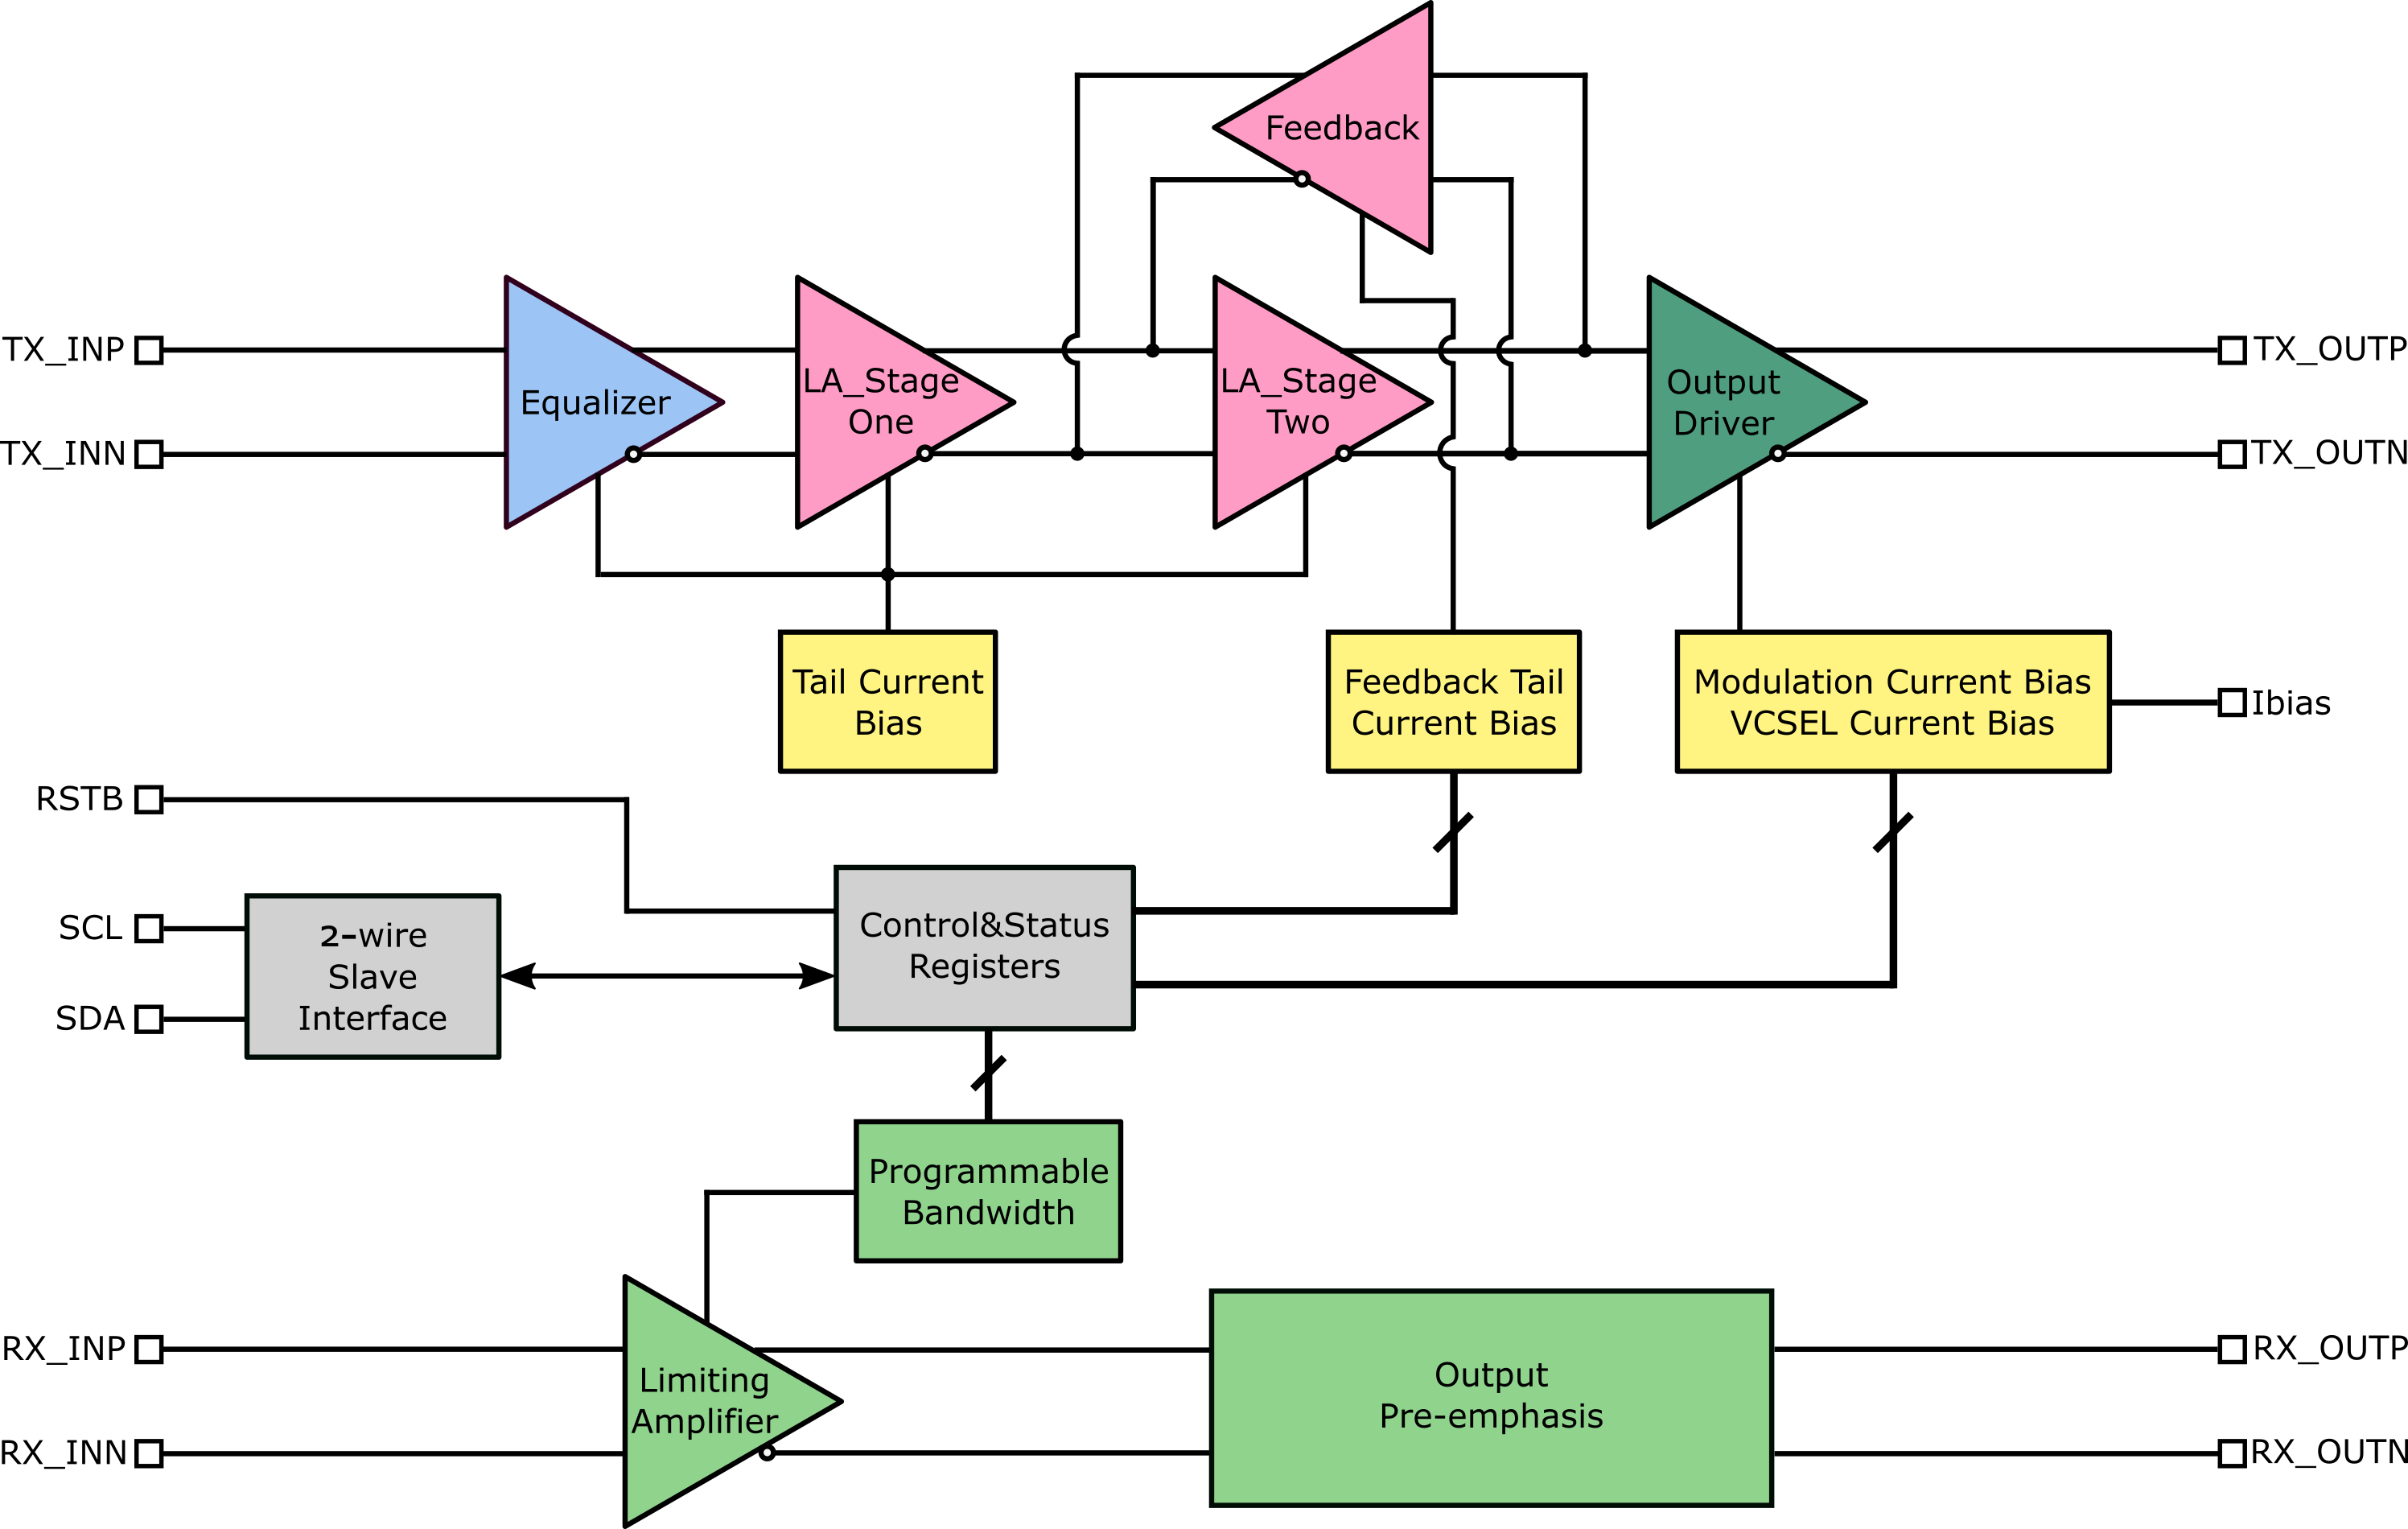
\includegraphics[width=\linewidth]{./Img/locld55.png}
    \caption{LOCld55 block diagram}
%    \lable{Figure 1}
\end{figure}
%Figure 1: LOCld55 block diagram

The die size and pad out of LOCld55 are shown in Section 2. Detailed schematic and layout designs are discussed in Section 3. The post-layout simulation results are introduced in Section 4.

\section{Pin Out of LOCld55}                % Part Two 

\subsection{Pin Assignment}

\subsection{Pin Descriptions}

\section{Detailed design of LOCld55}        % Part Three
\subsection{Equalizer}

\subsection{Limited Amplifier (LA)}

\subsection{Output Driver (OD)}

\subsection{Equalizer and Limited Amplifier biasing circuit}

\subsection{Modulation biasing circuit and Current biasing circuit}

\subsection{I2C}

\section{LOCld55 simulation results}        % Part Four

\subsection{Equalizer simulation results}

\subsection{Limiting Amplifier simulation results}

%\section{References}                        % Part Five

\end{spacing}

\bibliographystyle{plain}
\addcontentsline{toe}{chapter}{References}
\bibliography{LOCld55_Design_Document}

\end{document}
